\documentclass[12pt]{article}
\usepackage{graphicx}
%\documentclass[journal,12pt,twocolumn]{IEEEtran}
\usepackage[none]{hyphenat}
\usepackage{graphicx}
\usepackage{listings}
\usepackage[english]{babel}
\usepackage{graphicx}
\usepackage{caption} 
\usepackage{hyperref}
\usepackage{booktabs}
\def\inputGnumericTable{}
\usepackage{color}                                            %%
    \usepackage{array}                                            %%
    \usepackage{longtable}                                        %%
    \usepackage{calc}                                             %%
    \usepackage{multirow}                                         %%
    \usepackage{hhline}                                           %%
    \usepackage{ifthen}
\usepackage{array}
\usepackage{amsmath}   % for having text in math mode
\usepackage{listings}
\lstset{
language=tex,
frame=single, 
breaklines=true
}
  
%Following 2 lines were added to remove the blank page at the beginning
\usepackage{atbegshi}% http://ctan.org/pkg/atbegshi
\AtBeginDocument{\AtBeginShipoutNext{\AtBeginShipoutDiscard}}
%


%New macro definitions
\newcommand{\mydet}[1]{\ensuremath{\begin{vmatrix}#1\end{vmatrix}}}
\providecommand{\brak}[1]{\ensuremath{\left(#1\right)}}
\providecommand{\norm}[1]{\left\lVert#1\right\rVert}
\newcommand{\solution}{\noindent \textbf{Solution: }}
\newcommand{\myvec}[1]{\ensuremath{\begin{pmatrix}#1\end{pmatrix}}}
\let\vec\mathbf

\begin{document}


\begin{center}
\title{\textbf{Vector Algebra}}
\date{\vspace{-5ex}} %Not to print date automatically
\maketitle
\end{center}

\begin{enumerate}
\item\textbf{Problem statement :} The scalar product of the vector $\hat{i}+\hat{j}+\hat{k}$ with a unit vector along the sum of vectors $2\hat{i}+4\hat{j}-5\hat{k}$ and $\lambda\hat{i}+2\hat{j}+3\hat{k}$ is equal to one, Find the value of $\lambda$.
\\
\solution

Let
\begin{align}
\vec{a} =\myvec{1\\1\\1} , \vec{b}=\myvec{2\\4\\-5} , \vec{c}=\myvec{\lambda\\2\\3}
\end{align}
Then
\begin{align}
\brak{\vec{b}+\vec{c}}=\myvec{2\\4\\-5}+\myvec{\lambda\\2\\3}=\myvec{2+\lambda\\6\\-2}\\
{\norm{\vec{b}+\vec{c}}}={\sqrt{\lambda^2+4\lambda+44}}\\
\end{align}
Let $\vec{r}$ be the unit vector along with $\brak{\vec{b}+\vec{c}}$
\begin{align}
\hat{\vec{r}}=\frac{\brak{\vec{b}+\vec{c}}}{\norm{\vec{b}+\vec{c}}}
\end{align}
Given $\vec{a}^\top\brak{\vec{\hat{r}}} = 1$
\begin{align}
\vec{a}^\top\frac{\brak{\vec{b}+\vec{c}}}{\norm{\vec{b}+\vec{c}}}=1\\
\vec{a}^\top\brak{\vec{b}+\vec{c}}={\norm{\vec{b}+\vec{c}}}\\
\myvec{1&1&1}\myvec{2+\lambda \\ 6 \\ -2}= {\sqrt{\lambda^2+4\lambda+44}} \\
\lambda+6 = {\sqrt{\lambda^2+4\lambda+44}}\\
\end{align}
Squaring on both sides
\begin{align}
\brak{\lambda+6}^2 = \brak{{\sqrt{\lambda^2+4\lambda+44}}}^2\\
\lambda^2+12\brak{\lambda}+36 = \lambda^2+4\lambda+44\\
8\brak{\lambda} = 8\\
\lambda = 1
\end{align}
\begin{center}
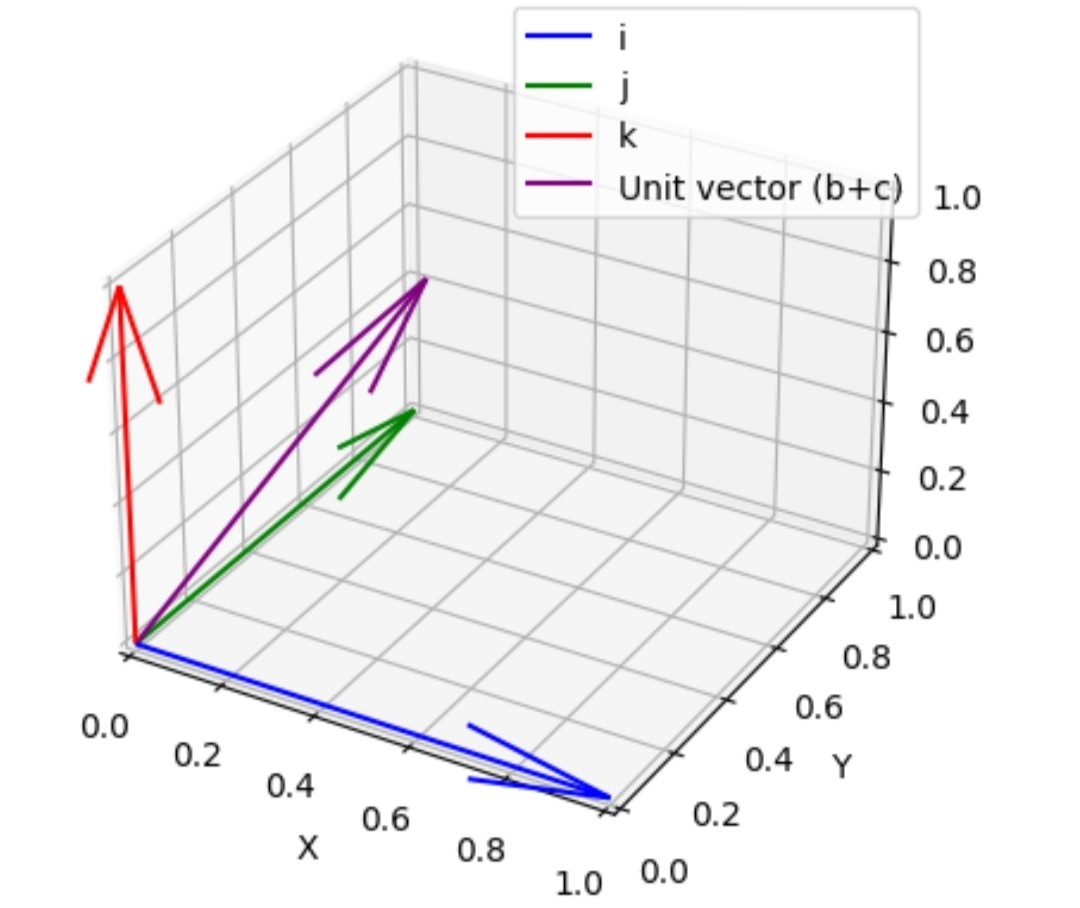
\includegraphics[width=\columnwidth]{figs/unitvector}
\end{center}
\end{enumerate}
\end{document}
